\documentclass[11pt, a4paper]{article}
\usepackage[utf8]{inputenc}
\usepackage[spanish,es-lcroman]{babel} 
\usepackage{graphicx}
\usepackage{mdframed}
\usepackage{enumitem}
\usepackage{xcolor}
\usepackage{hyperref}
\usepackage{amsmath, amssymb, amsfonts}
\usepackage{amsthm}
\usepackage{algorithm}
\usepackage{algpseudocode}
\usepackage{textcomp}
\usepackage{placeins}
\usepackage{etoolbox}
\usepackage{tikz}

\usetikzlibrary{decorations.pathreplacing}

\spanishdecimal{.}
\graphicspath{{images/}}
%COMILLAS “”
\title{Resumen Teórico Matemática Discreta II}
\author{Ferré Valderrama, Eduardo}
\date{\today}

\theoremstyle{definition}
\newtheorem{definition}{Definición}
\newtheorem{theorem}{Teorema}
\newtheorem{lemma}{Lema}
\newtheorem*{demostracion}{Demostración}
\newtheorem{corollary}{Corolario}
\newtheorem{proposition}{Proposición}
\newtheorem{example}{Ejemplo}
\newtheorem{exercise}{Ejercicio}
\newtheorem*{remark}{Observación}
\newtheorem{notation}{Notación}

%\qed(cuadradito vacio de que termino la demostración%
%\blacksquare(cuadradito lleno de que termino la demostración%

\begin{document}
\maketitle
Matemática Discreta II
\tableofcontents

\section{¿Cuál es la complejidad de Edmons-Karp?}

La complejidad del algoritmo de Edmons-Karp es $O(nm^2)$

\begin{demostracion}
    
    Para facilitar la prueba, supondremos que sí en el network está el lado $\overrightarrow{xy}$, 
    entonces no está el lado $\overrightarrow{yx}$.\\ \\
    Si $f_0, f_1, f_2, \ldots$ son los flujos parciales producidos al correr EK, entonces queremos ver que hay una cantidad finita de ellos y dar
    una cota para ese número. Como la búsqueda y construcción de cada camino aumentante se hace con \textbf{BFS}, cada incremento del flujo tiene 
    complejidad $O(m)$. \\ \\
    Así, que si probamos que sólo puede haber $O(nm)$ flujos aumentantes, tendremos la prueba de que la complejidad de EK es $O(nm^2)$.\\ \\
    Primero, decimos que un lado se vuelve crítico al pasar de $f_k$ a $f_{k+1}$ si se \textbf{satura} o \textbf{vacía}.\\ \\
    En cada construcción de un camino aumentante al menos un lado se vuelve crítico, el problema es que un lado puede volverse crítico muchas veces.
    Veamos cuantas veces puede pasar.\\ \\
    Supongamos que $\overrightarrow{xy}$ se vuelve crítico en el paso $k$, y luego en el paso $r$, con $r>k$. Tenemos que analizar dos casos:
    se vuelve crítico en el paso $k$ porque se saturó (llamemosle \textbf{Caso 1}), 
    o se vuelve crítico en el paso $k$ porque se vació, (a este caso lo llamamos \textbf{Caso 2}).\\ \\
    \begin{itemize}
        \item \textbf{Caso 1. En el que se satura (forward)}: Como se saturó en el paso $k$ entonces:
            \begin{itemize}
                \item Para construir $f_{k+1}$ se debe usar un $f_k$ camino aumentante de la forma $s \ldots \overrightarrow{xy} \ldots t$.
                \item Como estamos usando EK ese camino es de longitud mínima, por lo tanto: 
            \end{itemize}
                \begin{center}
                    $d_k(y)=d_k(x)+1$. \textbf{(1)}
                \end{center}
            Para que se vuelva crítico en el paso $r$, debe pasar una de estas dos cosas:
            \begin{itemize}
                \item Se vuelve crítico en el paso $r$ porque se vacía.
                \item Se vuelve crítico en el paso $r$ porque vuelve a saturarse.
            \end{itemize}
            Para que ocurra lo segundo, debe haberse vaciado antes aunque sea un poco, sino es imposible que vuelva a saturarse.\\ \\
            Entonces en cualquiera de estos dos casos, deducimos que existe $l$ tal que $k<l\leq r$ tal que el flujo en $\overrightarrow{xy}$ 
            disminuye al pasar de $f_l$ a $f_{l+1}$ ya sea vaciándose completamente o un poco.\\ \\
            Esto implica que para construir $f_{l+1}$ se usa un $f_l-$camino aumentante de la forma $s \ldots \overleftarrow{yx} \ldots t$.
            Como estamos usando EK, ese camino es de longitud mínima, por lo tanto:
                \begin{center}
                    $d_l(x)=d_l(y)+1$. \textbf{(2)}
                \end{center}
            Entonces:
            \begin{align*}
                d_l(t) &= d_l(x) + b_l(x). \\[6pt]
                &= d_l(y) + 1 + b_l(x) \quad \text{Por \textbf{(2)}} \\[6pt]
                &\geq d_k(y) + 1 + b_k(x) \quad \text{Porque las distancias no disminuyen} \\[6pt]
                &= d_k(x) + 1 + 1 + b_k(x) \quad \text{Por \textbf{(1)}} \\[6pt]
                &= d_k(t) + 2
                \end{align*}
                
                Este fue el análisis de si el lado $\overrightarrow{xy}$ se volvía crítico en el paso $k$ porque se saturaba. Ahora vamos con el 
                \textbf{Caso 2.}
            
        \item \textbf{Caso 2. En el que se vacía (backward)}: Como se vacía, existe un camino (de longitud mínima) de la forma 
                $s \ldots \overleftarrow{yx} \ldots t$ que se usa para pasar de $f_k$ a $f_{k+1}$. Por lo tanto:
                \begin{center}
                    $d_k(x)=d_k(y)+1$. \textbf{(3)}
                \end{center}
                Para que se vuelva crítico en el paso $r$, debe o bien volverse a vaciar, o bien saturarse, en el segundo de esos casos estamos 
                obviamente mandando más flujo en el paso $r$, pero en el primero si estamos diciendo que debe vaciarse de vuelta, entonces antes 
                debe haberse llenado aunque sea un poco. \\ \\ 
                Así que en cualquier caso debe haber un $l$ tal que $k<l\leq r$ para el cual se manda flujo a través de él. Entonces, existe un camino 
                (de longitud mínima) de la forma $s \ldots \overrightarrow{xy} \ldots t$ que se usa para pasar de $f_l$ a $f_{l+1}$. Por lo tanto:
                \begin{center}
                    $d_l(y)=d_l(x)+1$. \textbf{(4)}
                \end{center}
                Notemos que \textbf{(3)} y \textbf{(4)} son análogos a \textbf{(1)} y \textbf{(2)}, solo que con $x$ e $y$ intercambiados. 
                Entonces podemos deducir que $d_l(t) \geq d_k(t) + 2$ de la misma forma que en el \textbf{Caso 1}, simplemente intercambiando $x$ e $y$
                en la prueba. Así que también en este caso deducimos que $d_r \geq d_l(t) \geq d_k(t)+2$.\\ \\
                Entonces tanto como para el \textbf{Caso 1} como para el \textbf{Caso 2}, luego de que un lado se vuelva crítico, para que se vuelva 
                crítico otra vez, la distancia entre $s$ y $t$ debe aumentar al menos en 2. 
                
                Como la distancia entre $s$ y $t$ puede ir desde mínimo de $1$ hasta un máximo de $n-1$, entonces un lado puede volverse crítico 
                un máximo de \textbf{$O(\frac{n}{2}) = O(n)$ veces}.\\ \\
                Como cada camino aumentante que se usa en EK tiene al menos un lado que se vuelve crítico, entonces el total de flujos intermedios está
                acotado por $O(nm)$, puesto que hay $m$ lados y cada uno se puede volver crítico a lo sumo $O(n)$ veces.\\ \\
                Finalmente como cada construcción de un flujo tiene complejidad $O(m)$, entonces concluimos que la complejidad total de EK es 
                \begin{center}
                    $O(m)*O(nm) = O(nm^2)$ $\blacksquare$
                \end{center}     
    \end{itemize}
\end{demostracion}
\section{Probar que, si dados vértices $x,z$ y flujo $f$ definimos la distancia entre $x$ y $z$ relativa a $f$ como la longitud del menor
        $f$-camino aumentante entre $x$ y $z$, si es que existe tal camino, o infinito si no existe o 0 si $x=z$, denotándola por $d_f(x,z)$,
        y definimos $d_k(x)=d_{f_k}(s,x)$, donde $f_k$ es el $k$-ésimo flujo en una corrida de Edmonds-Karp, entonces $d_k(x)$ $\leq$ $d_{k+1}(x)$.}

\begin{demostracion}
    Vamos a demostrar que $d_k(x) \leq d_{k+1}(x)$.\\ \\
    Sea $A=\{y: d_{k+1}(y)<d_k(y)\}$. Queremos ver que $A=\emptyset$, supongamos que no.\\ \\
    Sea $x \in A$ tal que
    \begin{equation}
        d_{k+1}(x)=min\{d_{k+1}(y): y \in A\}
    \end{equation}
    Observemos que $x \in A$, entonces $d_{k+1}(x)<d_k(x) \leq \infty  \Rightarrow d_{k+1} < \infty$. Entonces existe un $f_{k+1}$-camino aumentante
    entre $s$ y $x$. 
    \begin{remark}
        $x \neq s$, pues $s\notin A$, pues $d_k(s)=d_{k+1}(s)=0$.
    \end{remark}
    Sea entonces $p_{k+1}:=s \ldots x$ un $f_{k+1}$-camino aumentante de longitud mínima entre $s$ y $x$, es decir, de longitud $d_{k+1}(x)$. Como 
    $x\neq s$ en ese camino existe un vertice inmediatamente anterior a $x$, llamemosle $z$. Entonces, $p_{k+1}=s \ldots zx$.\\
    Como $p_{k+1}$ es de longitud mínima entre $s$ y $x$, entonces es de longitud mínima entre $s$ y cualquier otro vertice intermedio como pej $z$. Por 
    lo tanto:
    \begin{equation}
        d_{k+1}(z)=d_{k+1}(x)-1
    \end{equation}
    Como $p_{k+1} = s \ldots zx$ es un $f_{k+1}$-camino aumentante, entonces existe el lado $\overrightarrow{zx}$ o existe el lado 
    $\overrightarrow{xz}$. Analicemos los dos casos.
    \begin{itemize}
        \item \textbf{Caso 1.} Si $\overrightarrow{zx}$ es un lado, tenemos que $d_{k+1}(z) < d_{k+1}(x)$. Pero
         
        \[ z \notin A \implies d_k(z) \leq d_{k+1}(z) < d_{k+1}(x) < \infty \]
        
        Como $d_k(z) < \infty$, existe un $f_k$-camino aumentante entre $s$ y $z$. 
        Lo denominamos $p_k$. Como $\overrightarrow{zx}$ es un lado, podría, en principio, agregar $x$ al final de $p_k$, 
        obteniendo un $f_k$-c.a. entre $s$ y $x$ que pasa por $z$. Pero entonces tendríamos 
        $d_k(x) \leq d_k(z) + 1 \leq d_{k+1}(z) + 1 \leq d_{k+1}(x)$. 
        Pero esto implica $x \notin A$. 
        
        Por lo tanto, no puedo agregar $x$ al final de $p_k$. 
        Entonces, o bien el lado $\overrightarrow{zx}$ está saturado en el paso $k$, o bien $f_k(\overrightarrow{zx}) = c(\overrightarrow{zx})$. 
        Pero $p_{k+1}$ era aumentante; es decir, sus lados no pueden estar saturados; 
        lo cual implica que $f_{k+1}(\overrightarrow{zx}) < c(\overrightarrow{zx})$ en el paso $k + 1$. 
        Luego, para pasar de $f_k$ a $f_{k+1}$, se usó el lado $\overrightarrow{xz}$ y se usó backwards en el camino
        
        \[ \tilde{p}_k : s \ldots \tilde{z} \ldots t \]
        
        Como este camino se usa en Edmonds-Karp, es de longitud mínima. Por lo tanto,
        
        \[ d_k(z) = d_k(x) + 1 \]
        \textbf{Completar, falta determinar el absurdo.}


        \item \textbf{Caso 2.} Si $\overrightarrow{zx}$ es un lado, tenemos que $p_{k+1}$ es de la forma $s \ldots zx$. Como antes, 
        \[ d_{k+1}(z) < d_{k+1}(x) \implies z \in A \implies d_k(z) \leq d_{k+1}(z) \]
        lo cual a su vez implica que existe un $f_k$-camino aumentante entre $s$ y $z$:
        \begin{center}
            $p_k: s \ldots z$
        \end{center}
        Podríamos agregar a $x$ en el final de este camino usando $\overrightarrow{xz}$ backward: llegaríamos a la misma contradicción que antes, en 
        que no podríamos agregar $x$. En este caso, si no lo podemos agregar, es porque $f_k(\overrightarrow{xz})=0$. Pero $p_{k+1}$ es 
        $f_{k+1}$-aumentante, lo cual implica que $f_{k+1}(\overrightarrow{xz})>0$. Luego debimos haber usado $\overrightarrow{xz}$ en modo forward al 
        pasar de $f_k$ a $f_{k+1}$. Por lo tanto existe un $f$-camino aumentante de la forma:
        \begin{center}
            $\tilde{p}_k: s \ldots \overrightarrow{xz} \ldots t$
        \end{center}
        Y luego como usamos Edmonds-Karp, este camino aumentante es de longitud mínima.\\
        Luego $d_k(z) = d_k(x) + 1$.\\
        \textbf{Completar, falta determinar el absurdo.}
    \end{itemize}
    Finalmente concluimos $A=\emptyset$, es decir, que $d_k(x) \leq d_{k+1}(x)$. $\blacksquare$
\end{demostracion}

\section{Probar que, si dados vértices $x,z$ y flujo $f$ definimos la distancia entre $x$ y $z$ relativa a $f$ como la longitud del menor
        $f$-camino aumentante entre $x$ y $z$, si es que existe tal camino, o infinito si no existe o 0 si $x=z$, denotándola por $d_f(x,z)$,
        y definimos $b_k(x)=b_{f_k}(x,t)$, donde $f_k$ es el $k$-ésimo flujo en una corrida de Edmonds-Karp, entonces $b_k(x)$ $\leq$ $b_{k+1}(x)$.}

\begin{demostracion}
    \textbf{Se evalúa en diciembre de 2024.}
\end{demostracion}

\section{¿Cual es la complejidad del algoritmo de Dinic? Probarla en ambas versiones: Dinitz original y Dinic-Even. 
(no hace falta probar que la distancia en networks auxiliares sucesivos aumenta).}
La complejidad de Dinitz, en su versión original como occidental, es $O(n^2m)$.

\begin{demostracion}
    Como el nivel de $t$ en los networks auxiliares aumenta, solo puede haber $O(n)$ networks auxiliares. 
    \(\therefore\)La complejidad de Dinitz es igual a la complejidad de hallar un flujo bloqueante en un network auxiliar, 
    más la complejidad de construir un network auxiliar, 
    por la cantidad de networks auxiliares---que es $O(n)$. 
    Porque usamos DFS, la complejidad de construir un network auxiliar es $O(m)$. 
    Entonces basta probar que la complejidad de hallar un flujo bloqueante es $O(nm)$, porque tendremos
    \[ O(n) \cdot (O(m) + O(nm)) = O(n^2m) \]

    \newpage

    \begin{itemize}
        \item \textbf{Versión Original: } \\ \\
        En la versión original del algoritmo, el n.a. es tal que no hay vértices sin lado de salida. Esto implica que DFS siempre llega a $t$ sin hacer backtracking. Entonces, DFS no es $O(m)$ sino $O$(cantidad de niveles) que podemos simplificar como $O(n)$. Como cada camino borra al menos un lado del n.a. hay $O(m)$ caminos. Luego la complejidad de hallar los caminos y aumentar el flujo por ellos es $O(nm)$. Pero debemos calcular el costo de que el n.a. satisfaga la propiedad de que no hay vértices sin lados de salida.

        Para esto, luego de cada camino hay que hacer algo para mantener esa propiedad como invariante. Dinitz llamó a la operación que logra esto \textbf{``podar''}. La operación consiste en recorrer los vértices desde los niveles más altos a los más bajos, chequea si el vértice tiene lados de salida; si tiene no hace nada, si no lo tiene lo borra.
        
        Chequear si el lado tiene lados de salida es $O(1)$; hay $O(n)$ vértices, y hay un ``podar'' por cada camino y hay $O(m)$ caminos. Esto entonces también es $O(nm)$.
        
        Nos queda analizar la complejidad de borrar el vértice y sus lados; esto se hace a lo sumo una vez por vértice, y una vez que podamos un vértice es probable que podar los siguientes requiera una complejidad menor (porque estamos quitando lados). Esto nos dice que podemos pensar en la complejidad promedio del problema, y no en la complejidad límite (es decir como cota).
        
        Borrar un vértice $x$ y sus lados es $O(d(x))$; sobre todos los vértices, esto da $\sum O(d(x)) = O(m)$ (por la propiedad del apretón de manos). Luego la complejidad de hallar un flujo bloqueante es:
        
        \[
        O(nm) + O(nm) + O(m) = O(nm) \blacksquare
        \]
        \item \textbf{Versión Dinic-Even: } \\
        Ahora consideremos la versión occidental. Lo más cómodo es dar el pseudocódigo. Estamos hablando del network auxiliar y el problema de hallar un flujo bloqueante en él.

        Para hallar flujo bloqueante $g$ en un n.a:
        \begin{algorithm}[!ht]
            \caption{Algoritmo}
            \begin{algorithmic}[1]
            \State $g := 0$
            \State $bool\ flag := true$
            \While{$flag$}
               \State type $path := [s]$
               \State $int\ x := s$
               \While{$x \neq t$}
                   \If{$\Gamma^+(x) \neq 0$}
                       \State tomar $y \in \Gamma^+(x)$
                       \State agregar $y$ a $path$
                       \State $x := y$ \Comment{Esta línea y la anterior son la parte (A) de avanzar}
                   \Else
                       \If{$x \neq s$}
                           \State $z :=$ elemento anterior a $x$ en $path$ \Comment{(R) Retroceder}
                           \State borro $x$ de $path$
                           \State borro $\overrightarrow{zx}$ de la n.a.
                           \State $x := z$
                       \Else
                           \State $flag := 0$
                       \EndIf
                   \EndIf
               \EndWhile
               \If{$x = t$}
                   \State aumentar flujo $g$ a lo largo de $path$ \Comment{(I) Incrementar}
                   \State borrar lados saturados
               \EndIf
            \EndWhile
            \State \textbf{return} $g$
            \end{algorithmic}
            \end{algorithm}
            \FloatBarrier

            Entonces, una corrida de Dinitz occidental es una palabra $AAAIAAARARRAA\ldots$
            Miraremos subpalabras de la forma $A\ldots AX$ con $X \in \{I, R\}$. 
            \begin{itemize}[noitemsep, nolistsep]
                \item Cada $A$ es $O(1)$;
                \item Cada $R$ es $O(1)$;
                \item Cada $I$ es recorrer un camino dos veces (una para incrementar el flujo, otra para borrar los lados), y resulta ser $O(n)$.
            \end{itemize}
            La cantidad de A's en $A\ldots AX$ se calcula como sigue. Cada avanzar, mueve el pivote
            $x$ de un nivel al siguiente. $\therefore$ Hay $O(n)$ letras A.
            \begin{itemize}[noitemsep, nolistsep]
                \item Cada avanzar, mueve el pivote $x$ de un nivel al siguiente. $\therefore$ Hay $O(n)$ letras A.
                \item $\therefore O(A\ldots AR) = O(n) + O(1) + O(n)$
                \item y $O(A\ldots AI) = O(n)(\#A) + O(n)(\#I) = O(n)$
            \end{itemize}
            Donde $\#Z$ es la cantidad de veces que ocurre la letra $Z$ en la palabra en cuestión. En
            resumen, $O(A\ldots AX) = O(n)$. Y la cantidad de palabras $A\ldots AX$ en una corrida se
            calcula así: 
            \begin{itemize}[noitemsep, nolistsep]
                \item Cada $R$ borra un lado, 
                \item y cada $I$ borra \textit{al menos} un lado;
                \item luego hay $O(m)$ palabras $A\ldots AX$.
            \end{itemize}
              Luego la complejidad total es $O(nm)$. $\blacksquare$
    \end{itemize}
\end{demostracion}


\section{¿Cual es la complejidad del algoritmo de Wave? Probarla.}
La complejidad de Wave es $O(n^3)$.

\begin{demostracion}
    Como es un algoritmo de tipo Dinitz, la distancia en n.a aumenta. Por lo tanto hay $O(n)$ networks auxiliares. Basta probar que la complejidad de 
    hallar un flujo bloqueante en Wave es $O(n^2)$.\\
    Dividiremos la complejidad en varias partes. 

    \begin{itemize}
        \item Los \textbf{“Los balanceos hacia adelante”} de los vertices.\\
                Cuando un vertice $x$ manda flujo a $z$, puede pasar que $\overrightarrow{xz}$ se sature o no. Sea entonces:
                \begin{itemize}
                    \item $S=$ Todos los pasos donde se satura un lado.
                    \item $P=$ Todos los pasos donde no se satura un lado.
                \end{itemize}
        \item Los \textbf{“Los balanceos hacia atrás”} el razonamiento es análogo.\\
                Cuando devolvemos flujo, podemos devolverlo todo o solo un poco. Sea entonces:
                \begin{itemize}
                    \item $V=$ La parte donde se vacían los lados.
                    \item $Q=$ La parte donde se devuelve flujo parcialmente.
                \end{itemize}
    \end{itemize}
    Entonces la complejidad de hallar un flujo bloqueante en Wave es 
    \begin{center}
        $S+P+V+Q$
    \end{center} 
    Analicemos cada una en detalle.

    \begin{itemize}
        \item \textbf{Análisis de $S$}\\
        Como habíamos mencionado, cuando un vertice $x$ manda flujo a $z$, puede pasar que $\overrightarrow{xz}$ se sature o no. Supongamos que 
        $\overrightarrow{xz}$ se saturó. La pregunta es si puede volver a saturarse en alguna ola hacia adelante. Para volver a saturarse, debe primero
        des-saturarse.
        \begin{center}
            Por lo tanto, $z$ debe devolverle flujo a $x$ $\Rightarrow$ $z$ debe estar “bloqueado”.
        \end{center} 
        Pero, en las olas hacia adelante, cuando un vértice chequea sus vecinos, solo se manda flujo a vertices no bloqueados. Entonces si $z$ le 
        devuelve flujo a $x$, $x$ no le puede volver a mandar flujo a $z$, por lo tanto:
        \begin{itemize}
            \item $\overrightarrow{xz}$ no se puede volver a saturar otra vez.
            \item Entonces cada lado se satura a lo sumo una vez.
        \end{itemize}
        Entonces concluimos que la complejidad de $S$ es $O(m)$.
        \item \textbf{Análisis de $V$}\\
        La pregunta es cuantas veces puede vaciarse un lado. La respuesta es muy similar al caso de $S$. 
        Si $x$ devuelve flujo a un vertice $u$ y se vacía $\overrightarrow{ux}$, entonces $x$ debe estar bloqueado, por lo tanto:
        \begin{itemize}
            \item $u$ nunca puede volver a enviar flujo.
            \item Por lo tanto, $\overrightarrow{ux}$ no puede volver a vaciarse (porque no se puede volver a enviar nada).
            \item Entonces cada lado se vacía a lo sumo una vez.
        \end{itemize}
        Entonces concluimos que la complejidad de $V$ es $O(m)$.
        \item \textbf{Análisis de $P$ y $Q$}\\
        Cuando intentamos balancear hacia adelante desde un vértice,
        todos los lados excepto quizas el ultimo se saturan. Es decir, en cada vértice de
        cada ola hacia adelante, hay a lo sumo un lado que no se satura, y "cuenta" para la
        complejidad de $P$. 
        \begin{itemize}
            \item Enviar flujo por ese lado es $O(1)$. 
            \item Luego la complejidad de $P$ es $O(n)$$*$$(\#$olas hacia adelante$)$.
        \end{itemize}
        Similar en $Q$.

        Al balancear hacia atras, en cada vértice se vacían todos los lados excepto a lo sumo uno. 
        \begin{itemize}
            \item Luego la complejidad de $Q$ es $O(n)$$*$$(\#$olas hacia atrás$)$.
        \end{itemize}
        Luego tenemos que:
        \begin{center}
            $\#$olas hacia adelante $=$ $\#$olas hacia atrás
        \end{center}
        Pues a cada ola hacia adelante corresponde una ola hacia atras. Ahora bien tenemos que calcular la cantidad de olas.

        En cada ola hacia adelante excepto la ultima (cuando se logra el balanceo), algun vertice queda desbalanceado. 
        Pero entonces la ola debio de bloquearlo. Por lo tanto, en cada ola hacia adelante excepto tal vez la ultima, 
        se bloquea al menos un vertice. Los vertices nunca se desbloquean.
        \begin{itemize}
            \item Luego hay $O(n)$ olas.
            \item Entonces la complejidad de $P$ es igual a la de $Q$
            \item Esto es $O(n)*O(n) = O(n^2)$
        \end{itemize}
        Finalmente tenemos que la complejidad de hallar un flujo bloqueante en Wave es:
        \begin{align*}
            S+P+V+Q &= O(m) + O(n^2) + O(m) + O(n^2) \\[6pt]
            &= O(n^2) + O(n^2) + O(m) + O(m) \\[6pt]
            &= O(n^2) + O(m) \quad \text{y} \quad m=O(n^2) \\[6pt]
            &= O(n^2) \blacksquare \\[6pt]
        \end{align*}    
    \end{itemize}
\end{demostracion}

\section{Probar que la distancia en networks auxiliares sucesivos aumenta.}
\textbf{Se evalúa en diciembre de 2024.}

\section{Probar que el valor de todo flujo es menor o igual que la capacidad de todo corte y que si $f$ es un flujo, entonces $f$ es
maximal si y solo si existe un corte $S$ tal que $v(f )=cap(S)$. (y en este caso, S es minimal)
(puede usar sin necesidad de probarlo que si $f$ es flujo y $S$ es corte entonces $v(f )=f(S,\overline{S})-f(\overline{S}, S)$)}


\textbf{Demostración.}
    \begin{enumerate}
        \item Probaremos que $f\leq Cap(S)$ para un corte $S$ y un flujo $f$ arbitrarios. Por lema sabemos que:
        \begin{center}
            $v(f)=f(S,\overline{S})-f(\overline{S},S)$
        \end{center}
        Observemos que el término $f(\overline{S},S)$ es de la forma $\sum f(\overrightarrow{xy})$. Por definición, cada término en esa sumatoria
        es mayor o igual a cero, y por lo tanto la sumatoria es positiva. Entonces tenemos que $-f(\overline{S},S) \leq 0$. Luego
        \begin{center}
            $v(f)=f(S,\overline{S})-f(\overline{S},S) \leq f(S,\overline{S})$
        \end{center}
        El primer término:$f(S,\overline{S})$, también es una sumatoria de términos positivos y es por lo tanto mayor a cero, pero cada término es 
        a su vez menor a la capacidad de cada lado, es decir $f(S,\overline{S})\leq c(S,\overline{S})=Cap(S)$. Por lo tanto:
        \begin{center}
            $v(f)\leq f(S,\overline{S})\leq Cap(S)$ $\blacksquare$
        \end{center}
        \item Ahora probemos que $f$ es maximal $\Longleftrightarrow$ existe un corte minimal $S$ tal que $v(f)=Cap(S)$.
        \begin{itemize}
            \item \textbf{($\Leftarrow$)} Sea ahora $f$ un flujo y $S$ un corte con $v(f)=Cap(S)$. Sea $g$ cualquier otro flujo. Entonces, por la 
                propiedad recien demostrada, $v(g)\leq Cap(S)$. Pues $Cap(S)=v(f)$, tenemos $v(g)\leq v(f)$. Por lo tanto $f$ es maximal. Como 
                detalle si $T$ es un corte, $Cap(T)\geq v(f)=Cap(S)$, lo cual implica que $S$ es minimal.
            \item \textbf{($\Rightarrow$)} Asumimos que \( f \) es maximal. Probaremos que existe un corte \( S \) con \( v(f) = C a p(S) \). 
            Para esto, debemos construir \( S \) a partir \( f \). Definiremos

            \[ S = \{s\} \cup \{ x \in V : \exists f\text{-camino aumentante entre } s \text{ y } x \} \]
            
            Que \( S \) es un corte se sigue por contradicción. Si \( S \) no es corte, debe contener a \( t \). 
            Luego existe un \( f\text{-camino aumentante desde } s \text{ a } t \). 
            Esto implica que puedo aumentar el flujo \( f \), lo cual contradice que \( f \) es maximal. 
            
            Sabiendo que \( S \) es un corte, tenemos
            
            \[ v(f) = f(S, \overline{S}) - f(\overline{S}, S) \tag{1} \]
            
            Consideremos el primer término en la resta de (1):
            
            \[ f(S, \overline{S}) = \sum_{\substack{x \in S \\ z \notin S \\ \overrightarrow{xz} \in E}} f(\overrightarrow{xz}) \]
            
            Sea \(\overrightarrow{xz}\) un par dentro del rango de la suma de arriba. 
            Pues \( x \in S \), existe un \( f\text{-camino aumentante de } s \text{ a } x \). 
            Pues \( z \notin S \), no existe un \( f\text{-camino aumentante de } s \text{ a } z \). 
            Pero el lado \(\overrightarrow{xz}\) sí existe. Así que \( s \ldots xz \) podría ser un \( f\text{-camino aumentante} \); 
            como tal camino no existe por hipótesis, no es aumentante. 
            Esto implica que \( f(\overrightarrow{xz}) = c(\overrightarrow{xz}) \). 
            La conclusión es que \( f(\overrightarrow{xz}) = c(\overrightarrow{xz}) \) para todo \( x \in S, z \notin S, \overrightarrow{xz} \in E \). 
            Entonces

            \[ f(S, \overline{S}) = \sum_{\substack{x \in S \\ z \notin S \\ \overrightarrow{xz} \in E}} f(\overrightarrow{xz}) = \sum_{\substack{x \in S \\ z \notin S \\ \overrightarrow{xz} \in E}} c(\overrightarrow{xz}) = Cap(S) \]

            Ahora consideremos el segundo término de la ecuación (1).

            \[ f(\overline{S}, S) = \sum_{\substack{w \notin S \\ x \in S \\ \overrightarrow{wx} \in E}} f(\overrightarrow{wx}) \]

            Sea \(\overrightarrow{wx}\) un par arbitrario en el rango de la suma. Como antes, \( x \in S \Rightarrow \) que hay un camino aumentante de \( s \) a \( x \); pero no existe camino aumentante entre \( s \) y \( w \); pero \(\overrightarrow{wx}\) es un lado. Es decir, \( s \ldots \overleftarrow{wx} \) podría ser un \( f\text{-camino aumentante}\); y como no lo es sucede que \( f(\overrightarrow{wx}) = 0 \). Luego

            \[ f(\overline{S}, S) = \sum_{\substack{w \notin S \\ x \in S \\ \overrightarrow{wx} \in E}} f(\overrightarrow{wx}) = 0 \]

            Luego \( v(f) = Cap(S) - 0 = Cap(S) \). \(\blacksquare\)
        \end{itemize}

    \end{enumerate}


\section{Probar que si $G$ es conexo no regular, entonces $\chi(G)\leq \Delta(G)$.}

Sea \( x \) tal que \( d(x) = \delta(G) \). Corro BFS empezando por \( x \) y guardo el orden inverso en que los vértices se visitaron. Ahora voy a correr greedy en este orden que acabo de guardar. Notar que en BFS todo vértice es incluido por un vértice que ya ha sido visitado, entonces en el orden inverso todo vértice tiene al menos un vecino por delante (excepto el \( x \)). Esto significa que para cada vértice \( y \), en el peor caso va a tener \( d(y) - 1 < \Delta \) vecinos coloreados todos con un color distinto, entonces voy a poder elegir un color en \(\{1, \cdots, \Delta\}\). Finalmente, cuando llego a \( x \), como \( d(x) = \delta < \Delta \), podré elegir algún color de \(\{1, \cdots, \Delta\}\) que no está usado por ningún vecino de \( x \) para colorearlo. De esta forma tengo un coloreo propio de \( G \) que usa (a lo sumo) \(\Delta\) colores, entonces \(\chi(G) \leq \Delta(G)\).

\section{Probar que 2-COLOR es polinomial}

\begin{demostracion}
    
    \textbf{Problema: "k-color":} 
    
    Dado $G$ ¿Es $\chi(G) \leq k$?, en particular $k=2$. 
    
    \begin{itemize}
        \item 1-color es trivial (no es polinomial).
        \item 2-color es polinomial (hay algún algoritmo que corre en tiempo polinomial en un rango de la entrada). 
        \item Entonces la idea de la demostración es correr un algoritmo en tiempo polinomial, en particular solo nos basta con correrlo en grafos conexos
    \end{itemize}
    Tomamos un $x \in V$, corremos BFS empezando en $x$. Si:
    \begin{align*}
        N(z) &= \text{nivel } z \text{ en el árbol BFS} \\[6pt]
             &= \text{distancia entre } z \text{ y } x \quad  \text{ en el árbol BFS} \\[6pt]
             &= \text{distancia entre } z \text{ y } x \quad  \text{ en } G \\[6pt]
    \end{align*}
    Sea:
    \begin{itemize}
        \item $C(z) = (N(z) \mod 2)$
        \item \textbf{If} ($C$ es propio, return si, es 2-colorable).
        \item \textbf{Else} (return no, no es 2-colorable).
    \end{itemize}
    El algoritmo es polinomial porque BFS es $O(m)$ y chequear que es propio es $O(m)$, lo que hay que probar es si es correcto. Entonces supongamos que la respuesta es \textbf{"no es 2-colorable"}.    
    \[
    \Rightarrow \exists v, z : c(v) = c(z) \land vz \in E
    \]

    Entonces $d(x, v) = d(x, z) \mod 2$\\
    Tomamos un camino entre $x$ y $v$ en BFS y un camino entre $x$ y $z$ en BFS y sea $w$ el único vértice en común (como lo muestra la siguiente figura).
    \begin{figure}[!ht]
        \centering 
        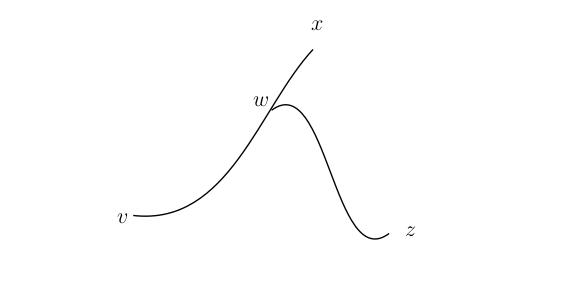
\includegraphics[height=6cm]{Figure 1 2-color.png} 
    \end{figure}

    Miramos el ciclo en $G$: $w \ldots \underset{\text{cruzo a }z}{\underbrace{vz}} \ldots \underset{\text{vuelvo a }x}{\underbrace{w}}$ (como lo muestra la siguiente imagen).

    \begin{figure}[!ht]
        \centering 
        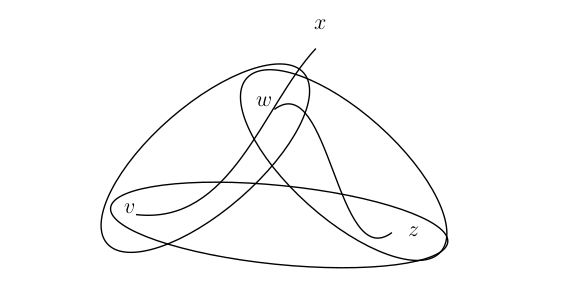
\includegraphics[height=6cm]{Figura 2 2-color.png} 
    \end{figure}
    Calculamos la longitud de este ciclo:
    \begin{align*}
    \text{longitud} &= 1 + d(v, w) + d(z, w) \\
    \text{longitud mod 2} &= (1 + d(v, w) + \ldots + d(z, w)) \text{ mod } 2 \\
    &= (1 + d(v, w) + d(z, w) + 2d(x, w)) \text{ mod } 2 \\
    &= (1 + d(x, v) + d(x, z)) \text{ mod } 2 = (1 + \overbrace{c(x) + c(z)}^{=0}) \text{ mod } 2 \\
    &= 1
    \end{align*}
    Es un ciclo impar, entonces no se puede colorear con 2 colores $\Rightarrow \chi(G)\geq 3. \blacksquare$
\end{demostracion}

\section{Enunciar y probar el Teorema de Hall.}

Sea $G=(V,E)$ bipartito con partes $X$ e $Y$. Existe un matching completo de $X$ a $Y$ si y solo si 
\begin{center}
    $|\Gamma(S)| \geq |S| \quad \forall S \subseteq X$
\end{center}
Notemos que un matching $M$ de $X$ a $Y$ es completo si y solo si $|M|=|X|$.
\textbf{Demostración.}\\
\textbf{($\Rightarrow$)}\\  
Sea $M$ un matching completo de $X$ a $Y$, este matching nos induce a una función inyectiva
\begin{center}
    $f: X \rightarrow Y$
\end{center}
tal que 
\begin{center}
    $f(x)\in \Gamma(x)$
\end{center}
Como $f$ es inyectiva tenemos que:
\begin{center}
    $|f(S)|=|S| \quad \forall S \subseteq X$
\end{center}
Finalmente 
\begin{center}
    $f(S) \subseteq \Gamma(S) \Rightarrow |S| \leq |\Gamma(S)| \quad \forall S \subseteq X$
\end{center}
\textbf{($\Leftarrow$)}\\ 
Supongamos que se cumple la condición de Hall, es decir: 
\begin{center}
    $|\Gamma(S)| \geq |S| \quad \forall S \subseteq X$
\end{center}
Y también asumamos que al correr el algoritmo para hallar un matching maximal, llegamos a un matching maximal $M$ tal que
$|E(M)| < |X|$. Es decir, un matching incompleto en $X$ (podría ser en $Y$). Construiremos un $S \subseteq X$ que viola la condición de Hall, es decir tal que
\begin{center}
    $|\Gamma(S)| < |S|$
\end{center}
llegando a un absurdo.\\
Corramos el algoritmo de extensión de matching sobre el ultimo matching $M$. Como esta matching no cubre a $X$, existen filas sin matchear, más otras filas etiquetadas.
Entonces sean:
\begin{align*}
    S & = \{\text{\small filas etiquetadas}\} \\
    T & = \{\text{\small columnas etiquetadas}\} \\
    S_0 & = \{\text{\small filas etiquetadas con }*\} \\
    T_1 & = \{\text{\small columnas etiquetadas por }S_0\} \\
    S_1 & = \{\text{\small filas etiquetadas por } T_1\}
 \end{align*}
Y en general:
\begin{align*}
    T_{i+1} & = \{\text{\small columnas etiquetadas por }S_i\} \\
    S_i & = \{\text{\small filas etiquetadas por } T_i\}.
    \end{align*}
Notemos que como $M$ no es completo, tenemos algunas filas sin matchear, es decir que
\[S_0 \ne \emptyset \tag{0}\]
Las sucesiones son finitas y $S=S_0 \cup S_1 \cup \ldots$ con uniones disjuntas, y $T=T_1 \cup T_2 \cup \ldots$ con uniones disjuntas.\\
Cuando revisamos una columna pueden pasar dos cosas:
\begin{itemize}
    \item La columna está libre, entonces la matcheamos y extendemos el matching. Esto no pasa porque $M$ es maximal.
    \item La columna está matcheada con una fila, entonces etiquetamos únicamente esa fila.
\end{itemize}
Por lo tanto, el algoritmo nunca se detiene cuando pasa de algún $T_i$ a $S_i$. Es decir que el algoritmo se detiene solamente al pasar de un $S_k$ a un $T_{k+1}=\emptyset$\\
Observemos que, como cada columna etiqueta a la fila con la cual está matcheada, cada columna etiquetada etiqueta a una sola fila, entonces tenemos que:
\[|T_i|=|S_i| \tag{1}\]
Porque el $T_i$ crea al $S_i$\\ 
Y tambíen\\ 
$S=S_0 \cup S_1 \cup \ldots S_k$ con uniones disjuntas, y $T=T_1 \cup T_2 \cup \ldots T_k$ con uniones disjuntas.\\ 
Entonces finalmente tenemos que:
\begin{align*}
    |S| & = |S_0| + |S_1| + \cdots + |S_k| \\
        & = |S_0| + |T_1| + \cdots + |T_k| \quad\text{por (1)} \\
        & = |S_0| + |T| > |T| \quad\text{por (0)} 
\end{align*}
Por lo tanto $|S| > |T|$. Ahora demostremos que $T=\Gamma(S)$.
\begin{itemize}
    \item \(T \subseteq \Gamma(S)\): sea \(y \in T\), \(y\) tuvo que ser etiquetado por una fila de S, y como cada fila etiqueta a sus columnas vecinas es claro que \({y \in \Gamma(S).}\)
    \item \(\Gamma(S) \subseteq T\): Supongamos que existe un \(y \in \Gamma(S)\) que no está en T. Existe un \({x \in S}\) que es vecino de \(y\). Pero cuando revisamos \(x\), habríamos visto que \(y\) era vecino suyo, y por lo tanto lo habríamos etiquetado. Absurdo pues habíamos supueto \({y \not\in T}\), luego, \({\Gamma(S) \subseteq T.}\)
\end{itemize}
    
Finalmente, construimos un \(S \subseteq X\) tal que no se cumple la condición de Hall. Lo que es un absurdo pues habiamos supuesto que era cierta. Entonces este absurdo viene de suponer que el matching maximal no es completo.$\blacksquare$

\section{Enunciar y probar el teorema del matrimonio de Koenig}

Todo grafo bipartito regular tiene matching perfecto.

\begin{demostracion}
Dado $W \subseteq V$, definimos
\[
E_W = \{wu : w \in W\}
\]
Sean $X, Y$ las partes de $G$. Sea $S \subseteq X$. Sea $l \in E_S$. Se sigue que
\[
\exists x \in S, y \in Y : l = xy = yx
\]
Es decir que $y \in \Gamma(x)$. Pero $x \in S$. Entonces $y \in \Gamma(S)$. Entonces $l \in E_{\Gamma(S)}$. $\therefore E_S \subseteq E_{\Gamma(S)}$. Por lo tanto
\[
|E_S| \leq |E_{\Gamma(S)}| \tag{1}
\]
Calculemos en general $|E_W|$ cuando $W \subseteq X$ o $W\subseteq Y$. Si $wu \in E_W$, entonces $v \notin W$, pues $W \subseteq X \Rightarrow v \in Y$, $W \subseteq Y \Rightarrow v \in X$.\\
De lo anterior se sigue que
\[
E_W = \bigcup_{w \in W} \{wv : v \in \Gamma(w)\} \tag{2}
\]
donde la unión es disjunta. Luego
\[
|E_W| = \sum_{w \in W} |\Gamma(w)| = \sum_{w \in W} d(w) \tag{3}
\]
Como $G$ es regular, $d(w) = \delta = \Delta$. Luego
\[
|E_W| = \Delta |W| \tag{4}
\]
Usando (1) y (4) tenemos que
\[
|S| \Delta \leq |\Gamma(S)| \Delta \Rightarrow |S| \leq |\Gamma(S)| \tag{5}
\]
Como esto vale para todo $S \subseteq X$, el teorema de Hall implica que existe un matching completo de $X$ a $Y$. Si demostramos que $|X| = |Y|$, se seguirá que ese matching será perfecto.\\ \\
La primera forma de probar esto es ver que como $X, Y$ son las partes de $G, E = E_X = E_Y$. Entonces $|E_X| = |E_Y|$, de lo cual se sigue que $\Delta |X| = |Y| \delta \Rightarrow |X| = |Y|$.\\ \\
Otra forma de verlo es observar que, dado que existe un matching completo de $X$ a $Y, |X| \leq |Y|$. Pero la elección de $X$ sobre $Y$ en la prueba fue arbitraria. Por lo tanto vale lo mismo para $Y$. Luego $|X| = |Y|$.\\ \\
En ambos casos, el matching es perfecto. $\blacksquare$
\end{demostracion}

\section{Probar que si $G$ es bipartito entonces $\chi'(G) = \Delta(G)$.}
\textbf{Se evalua en diciemre de 2024}

\section{Probar la complejidad $O(n^4)$ del algoritmo Hungaro y dar una idea de como se la puede reducir a $O(n^3)$}
\textbf{Se evalua en diciemre de 2024}

\section{Enunciar y probar el teorema de la cota de Hamming}

Para todo código $C \in \{0,1\}^n$ con $\delta(c)=\delta$ y $t=\left\lfloor\frac{\delta-1}{2}\right\rfloor$ entonces:
\[
|C| \leq \frac{2^n}{1 + n + \binom{n}{2} + \cdots + \binom{n}{t}}
\]
\begin{demostracion}
Sea
\[
A = \bigcup_{v \in C} D_t(v)
\]
Buscamos $|A|$.\\ \\
Como $C$ corrige $t$ errores tenemos que
\[
D_t(v) \cap D_t(w) = \emptyset, \forall v, w \in C \text{ tales que } v \neq w
\]
Es claro que $A$ es unión disjunta\\
Ahora definimos
\[
S_r(v) = \{w \in C : d_H(v, w) = r\}
\]
De esta forma es claro que:
\[
D_t(v) = \bigcup_{r=0}^t S_r(v) \quad \text{unión disjunta}
\]
Sea $w \in S_r(v)$, hay un subconjunto de los $n$ bits de las palabras que tiene $r$ elementos tal que $w$ difiere de $v$ en esos $r$ bits. Entonces tenemos:
\begin{itemize}
    \item Dado $w \in S_r(v)$, podemos obtener $r$ bits en los que $v$ y $w$ difieren.
    \item Dado un conjunto de $r$ bits, podemos obtener un $w$ tal que $d_H(v,w) = r$
\end{itemize}
Así, existe una biyección entre $S_r(v)$ y el conjunto de subconjuntos de $r$ bits. Entonces la cardinalidad de estos conjuntos es la misma. Luego
\[
|S_r(v)| = \binom{n}{r} \implies |D_t(v)| = \sum_{r=0}^t \binom{n}{r}
\]
Finalmente tenemos:
\begin{align*}
    |A| & = \sum_{v\in C} |D_t(v)| \\
        & = \sum_{v\in C} \sum_{r=0}^t \binom{n}{r} \\
        & = |C| \sum_{r=0}^t \binom{n}{r} \\
        & \leq 2^n \quad \text{pues } A \subseteq \{0,1\}^n \implies |C| \leq \frac{2^n}{\sum_{r=0}^t \binom{n}{r}} \blacksquare
\end{align*}
\end{demostracion}
\section{Sea $C$ un código lineal con matriz de chequeo $H$. Entonces $\delta(C)$ es el mínimo número de columnas LD de $H$}
\textbf{Demostración.}\\
Sea
\(m = \min \{r : \exists r \text{ columnas LD de } H\}\).
Probaremos \(m = \delta(C)\).\\
Para ello probaremos que $\delta(C) \leq m$ y $\delta(C) \geq m$.\\
Denotaremos la $j$-ésima columna de $H$ como $H^(j)$.\\ \\
Por definición de $m$ existe $j_1, j_2, \ldots, j_r$ tal que $H^{(j_1)}, H^{(j_2)}, \ldots, H^{(j_r)}$ son LD.\\ \\
Entonces existen $c_1, c_2, \ldots, c_r$ no todos 0 tales que:
\[
c_1H^{(j_1)} + c_2H^{(j_2)} + \cdots + c_rH^{(j_r)} = 0
\]
Sea $e_i = (0, 0, \ldots, 1, \ldots, 0)$ con 1 en la posición $i$. Entonces: 
\[
    He_i^t = \left[
        \begin{array}{c}
        \hspace{8mm} i \hspace{8mm} \\
        \vdots \\
        \hspace{8mm} i \hspace{8mm} \\
        \vdots \\
        \hspace{8mm} i \hspace{8mm}
        \end{array}
        \right]
        \begin{bmatrix}
        0 \\
        \vdots \\
        1 \\
        \vdots \\
        0
        \end{bmatrix} = H^{(i)}
\]
Es la columna $i-$ésima de $H$.
\newpage
Sea $x = c_1e_{j_1} + c_2e_{j_2} + \cdots + c_re_{j_r}$, como no todos los $c_j$ son 0 entonces $x \neq 0$, por lo que:
\begin{align*}
    H x^t &= H(c_1 e_{j_1}^t + c_2 e_{j_2}^t + \cdots + c_r e_{j_r}^t) \\
          &= c_1 H e_{j_1}^t + c_2 H e_{j_2}^t + \cdots + c_r H e_{j_r}^t \\
          &= c_1 H^{(j_1)} + c_2 H^{(j_2)} + \cdots + c_r H^{(j_r)} = 0 \\
          &\Rightarrow H x^t = 0
\end{align*}

$\Rightarrow x \in C$ pues $C = Nu(H)$, pero su peso es $\leq m$, pues es suma de a lo sumo $m$ vectores de peso 1.
y vimos que $x \neq 0$ entonces sabemos que:
\[
\delta(C) = \min \{ |v| : v \in C, v \neq 0 \}
\]

\[
\text{Por lo tanto como } x \in C \text{ y } x \neq 0, \text{ entonces } x \text{ está en ese conjunto, así que tenemos:}
\]

\[
\delta(C) = \min \{ |v| : v \in C, v \neq 0 \} \leq |x|
\]
Pero su peso es $\leq m$, entonces:
\[
\delta(C) = \min \{ |v| : v \in C, v \neq 0 \} \leq |x| \leq m
\]
Entonces, $\delta(C) \leq m$.\\ \\
Ahora probaremos que $\delta(C) \geq m$.\\
Sea $x \neq 0 : \delta(C) = |x|$ entonces:
\begin{align*}
    x &= c_1 e_{i_1} + \ldots + c_{\delta(C)} e_{i_{\delta(C)}} \\
      &= 0 \quad \{\text{como} \text{ } x \in C, \text{entonces} \text{ } x \neq 0\} \\
      &= H x^t = H^{(i_1)} + \ldots + H^{(i_{\delta(C)})} \\
      &\Rightarrow \{H^j, \ldots H^{i_{\delta(C)}}\} \text{son LD} \implies \delta(C) \geq m 
\end{align*}
$\blacksquare$

\section{Sea $C$ un código cíclico de dimensión $k$ y longitud $n$ y sea $g(x)$ su polinomio generador. Probar i, ii, iii y iv}
\begin{enumerate}[label=\roman*.]
    \item $C$ está formado por los multiplos de $g(x)$ de grado menor que $n$:
    \[
    C = \{p(x) : gr(p) < n\&g(x)|p(x)\}
    \]
    \item $C = \{v(x) \odot g(x): v \text{ } \text{es un polinomio cualquiera} \}$ 
    \item $gr(g(x)) = n - k$
    \item $g(x)$ divide a $1 + x^n$
\end{enumerate}
\textbf{Demostración}
\subsubsection*{Prueba de i. y ii.}

Sea $C_1 = \{p(x) : gr(p) < n\&g(x)|p(x)\}$ y $C_2 = \{v(x) \odot g(x): v \text{ } \text{es un polinomio cualquiera} \}$.\\ 
Vamos a demostrar que $C \subseteq C_1$, $C_2 \subseteq C$ y $C_1 \subseteq C_2$.\\ \\
$\boldsymbol{C_1 \subseteq C_2}$\\ \\
Sea $p(x) \in C_1$, queremos ver si está en $C_2$. Entonces existe $q(x)$ tal que $p(x) = g(x) \cdot q(x)$, además:
\[
n > gr(p) = gr(g(x) \cdot q(x)) 
\]
Luego tomando modulo tenemos que 
\begin{align*}
    p(x) \mod (1 + x^n) &= g(x) \cdot q(x) \mod (1 + x^n) \\
                        &= g(x) \odot q(x) \in C_2  
\end{align*} 
Por lo tanto $p(x) \in C_2$.\\ \\
$\boldsymbol{C_2 \subseteq C}$\\ \\
$\text{Sea } p(x) = v(x) \odot g(x) \in C_2, \text{ con } v(x) \text{ un polinomio cualquiera de la forma}$
\[
v(x) = v_0 + v_1 \cdot x + v_2 \cdot x^2 + \cdots + v_{gr(v)} \cdot x^{gr(v)}
\]
Queremos ver que $p(x) \in C$. Entonces:
\begin{align*}
    p(x) &= v(x) \odot g(x) \\
    &= (v_0 + v_1 \cdot x + v_2 \cdot x^2 + \cdots + v_{gr(v)} \cdot x^{gr(v)}) \odot g(x) \\
    &= v_0 \odot g(x) + v_1 \cdot (x \odot g(x)) + v_2 \cdot (x^2 \odot g(x)) + \cdots + v_{gr(v)} \cdot (x^{gr(v)} \odot g(x)) \\
    &= v_0 \cdot g(x) + v_1 \cdot Rot(g(x)) + v_2 \cdot Rot^2(g(x)) + \cdots + v_{gr(v)} \cdot Rot^{gr(v)}(g(x)) \\
    &\in C
\end{align*}  
Ya que todas las rotaciones de $g(x)$ están en $C$, entonces $p(x) \in C$.
\newpage
$\boldsymbol{C \subseteq C_1}$\\ \\
Sea $p(x) \in C$, como las palabras de $C$ tienen longitud $n$, entonces $gr(p) < n$. Nos queda ver que $g(x)|p(x)$. Para ello dividamos $p$ por $g$:
\[
\exists q(x), r(x) : p(x) = g(x) \cdot q(x) + r(x) \quad \text{ con } gr(r) < gr(g)
\]
Ahora tomemos modulo:
\begin{align*}
    p(x) &= p(x) \mod (1 + x^n) \\
         &= (g(x) \cdot q(x) + r(x)) \mod (1 + x^n) \\
         &= g(x) \odot q(x) + (r(x) \mod (1 + x^n)) \\
         &= g(x) \odot q(x) + r(x) \quad \text{pues } gr(r) < gr(g) < n
\end{align*}
Por lo tanto tenemos que:
\[
r(x) = p(x) + g(x) \odot q(x)
\]
Y como $p \in C$ y $g(x) \odot q(x) \in C_2$, entonces $r(x) \in C$.\\
Pero como $g$ es el generador, este es el único polinomio no nulo de menor grado en $C$, y como $g(r) < gr(g)$, entonces $r(x) = 0$.\\
Finalmente, como $g(x)|p(x)$, entonces $p(x) \in C_1$.
\subsubsection*{Prueba de iii.}
Sea \(p(x) \in C\), entonces existe \(q(x)\) tal que \({ p(x) = g(x) \cdot q(x) .}\)\\ 
Además \({n > gr(p) = gr(g) + gr(q) }\), entonces \({ gr(q) < n - gr(g) .}\)\\
Ahora, sea un \(q(x)\) tal que \(gr(q) < n - gr(g)\), tenemos que \({ g(x) \cdot q(x) \in C. }\)\\ \\
Es decir, hay una biyección entre \(C\) y el conjunto de polinomios de grado menor a \({n - gr(g).}\) Entonces:
\begin{align*}
	|C| & = |\text{conjunto de polinomios de grado menor a } n - gr(g)| \\
      \iff & \\
  2^k & = 2^{n - gr(g)} \\
      \iff & \\
    k & = n - gr(g) \\
      \iff & \\
    gr(g) & = n - k \\
\end{align*}

\subsubsection*{Prueba de iv.}
Dividimos \(1+x^n\) por \(g(x)\):
\[ 
\exists q(x), r(x) : 1 + x^n = g(x) \cdot q(x) + r(x) \quad \text{ con } gr(r) < gr(g)
\]
Ahora, si tomamos módulo:
\begin{align*}
	0 & = (1 + x^n) \text{ mod } (1 + x^n) \\
    & = g(x) \cdot q(x) + r(x) \text{ mod } (1 + x^n) \\
    & = g(x) \odot q(x) + (r(x) \text{ mod } (1 + x^n)) \\
    & = g(x) \odot q(x) + r(x) \quad\text{pues } gr(r) < gr(g) < n \\
    &\Rightarrow r(x) = g(x) \odot q(x) \in C
\end{align*}
Pero como $g$, es el polinomio de $C$ no nulo de menor grado y \({gr(r) < gr(g),}\) entonces \({r(x) = 0}\) y \({g(x) | (1 + x^n).}\). $\blacksquare$


\section{Probar que 3SAT es NP-completo}



\section{Probar que 3COLOR es NP-completo}
Para probar esto, sabiendo que 3SAT es NP completo, demostraremos que 3SAT se reduce polinomialmente a 3COLOR.\\
Es decir, debemos, dada una instancia de 3SAT, es decir, una expresion booleana $B$ en CNF con exactamente 3 literales
por disjuncion, crear polinomialmente una instancia de 3COLOR, es decir, un grafo $G$, tal que $B$ es satisfacible si y solo si $G$
se puede colorear con 3 colores.\\ \\
Sean $x_1 \ldots x_n$ las variables de $B$ y $D_j$ disjunciones cada una con tres literales tales que:
\[
B = D_1 \land D_2 \land \ldots \land D_m
\]
Como cada $D_j$ tiene 3 literales, sean $\ell_{jr}$, $r = 1, 2, 3$ los 3 literales de $D_j$. Es decir, $D_j = \ell_{j1} \vee \ell_{j2} \vee \ell_{j3}$.\\ \\
Construiremos ahora $G$.\\
Primero daremos los vertices de $G$:
\begin{itemize}
    \item Tendremos para cada $i = 1, 2, \ldots, n$ dos vértices $u_i$, $w_i$.
    \item Además, para cada $j = 1, \ldots, m$ tendremos 6 vértices $a_{j1}$, $a_{j2}$, $a_{j3}$, $e_{j1}$, $e_{j2}$, $e_{j3}$.
    \item Finalmente, dos vértices especiales, que llamaremos el CAPITAN y el AVISPON.
\end{itemize}
Observemos que la construcción de los vértices es directa a partir de solamente saber $n$ y $m$ y es polinomial.
\newpage
Ahora daremos los lados\\
Para poder definir los lados, debemos definir una función $v$ del conjunto de literales $\{x_1, .., x_n, \neg x_1, ..., \neg x_n\}$ en el conjunto
$\{u_1, w_1, ..., u_n, w_n\}$ de la siguiente forma:
\[
v(x_i) = u_i \quad v(\neg x_i) = w_i
\]
Es decir, $v$ de un literal es $u_i$ si el literal es la $i$-ésima variable, y $w_i$ si el literal es la $i$-ésima negación de una variable.\\
Entonces definimos los siguientes lados:
\begin{itemize}
    \item Triángulos $\{a_{j1}a_{j2}, a_{j2}a_{j3}, a_{j1}a_{j3}\}$, $j = 1, .., m$.
    \item Unir bases con extremos: $a_{jr}e_{jr}$, $j = 1, .., m$, $r = 1, 2, 3$. (Nota: los triángulos anteriores más estos últimos lados se
    llaman las “garras” porque al dibujarlos parecen unas garras).
    \item Unir extremos con el CAPITAN: $CAPITAN e_{jr}$, $j = 1, .., m$, $r = 1, 2, 3$.
    \item Triángulos basados en el avispon: $AVISPON u_i$, $AVISPON w_i$, $u_i w_i$, $i = 1, \ldots, n$.
    \item $(CAPITAN)(AVISPON)$ es otro lado.
    \item Lados $e_{jr}v(\ell_{jr})$, $j = 1, .., m$, $r = 1, 2, 3$.
\end{itemize}
Los primeros 4 tipos de lados dependen solo de $n$ y $m$, son los últimos lados los que capturan la “estructura” de $B$.\\
Está claro que la construcción es polinomial, porque solo leemos quiénes son $n$, $m$ y los literales $\ell_{jr}$ para construir $G$ y el
número de vértices y lados es lineal en estos números.\\ \\
Como $G$ tiene triángulos, sabemos que $\chi(G) \geq 3$. Demostremos entonces que $B$ es satisfacible si y solo si $\chi(G) = 3$.
\subsubsection*{$B$ es satisfacible $\Rightarrow \chi(G) = 3$}
Como $B$ es satisfacible, existe $\vec{b}$ un vector de bits tal que $B(\vec{b}) = 1$.\\
Colorearemos $G$ a partir de $\vec{b}$, y cada vez que coloreemos un vértice o conjunto de vértices debemos asegurarnos que el
coloreo sigue siendo propio.\\
Para empezar definimos:
\begin{itemize}
    \item Color del CAPITAN: ESCARLATA
    \item Color del AVISPON: VERDE
    \item Entonces el lado $(CAPITAN)(AVISPON)$ no crea problemas porque sus extremos tienen colores distintos.
\end{itemize}
Luego definimos:
\begin{itemize}
    \item Color de $u_i$ = ESCARLATA si $b_i = 1$ y NEGRO si $b_i = 0$.
    \item Color de $w_i$ = ESCARLATA si $b_i = 0$ y NEGRO si $b_i = 1$.
\end{itemize}
Entonces cada triángulo $AVISPON u_i$, $AVISPON w_i$, $u_i w_i$ tienen los colores VERDE, ESCARLATA y NEGRO en algún
orden, así que no crea problemas.\\ \\
Todavía no usamos que $B(\vec{b}) = 1$. Esa propiedad implica que $D_j(\vec{b}) = 1$ para todo $j$, y como $D_j$ es una disyunción eso
implica que:
\[
\forall j \in \{1, \ldots, m\} \exists r_j \in \{1, 2, 3\} : \ell_{jr_j}(\vec{b}) = 1
\]
(Si hay más de un “$r_j$“ elegimos uno solo)\\
Entonces coloreamos, para cada $j = 1, \ldots, m$:
\begin{itemize}
    \item Color de $a_{jr_j}$: VERDE
    \item Color de $a_{jk}$ para $k \neq r_j$: Uno NEGRO y el otro ESCARLATA.
\end{itemize}
De esta forma los triángulos $a_{j1}a_{j2}$, $a_{j2}a_{j3}$, $a_{j1}a_{j3}$ no crean problemas porque sus vértices tienen los tres colores distintos.\\
Luego coloreamos los extremos:
\begin{itemize}
    \item Color de $e_{jr_j}$: NEGRO
    \item Color de $e_{jk}$ para $k \neq r_j$: VERDE
\end{itemize}
Entonces:
\begin{itemize}
    \item Los lados $a_{jr_j}e_{jr_j}$ no crean problemas porque uno de sus extremos es VERDE y el otro NEGRO.
    \item Y para $k \neq r_j$, los lados $a_{jk}e_{jk}$ no crean problemas porque uno de sus extremos es NEGRO o ESCARLATA y el otro VERDE.
    \item Además los lados $CAPITAN e_{jk}$ ($k = 1, 2, 3$) no crean problemas porque el color del CAPITAN es ESCARLATA y el de los $e_{jk}$ es NEGRO o VERDE.
    \item Los lados $e_{jk}v(\ell_{jk})$ para $k \neq r_j$ no crean problemas porque el color de $e_{jk}$ es VERDE para esos $k$, mientras que el color
    de $v(\ell_{jk})$, que será un $u_i$ o $w_i$, va a ser NEGRO o ESCARLATA.
    \item Finalmente, quedan los lados $e_{jr_j}v(\ell_{jr_j})$. El color de $e_{jr_j}$ es NEGRO así que acá podría haber algún problema. Lo que
    debemos probar para evitar el problema es que el color de $v(\ell_{jr_j})$ es ESCARLATA.
\end{itemize}
Para probar esto, debemos analizar qué tipo de literal es $\ell_{jr_j}$:
\begin{enumerate}
    \item Si $\ell_{jr_j}$ es una variable:\\
    \begin{itemize}
        \item Entonces existe $i$ tal que $\ell_{jr_j} = x_i$.
        \item $\ell_{jr_j} = x_i$ implica por definición de $v$ que $v(\ell_{jr_j}) = u_i$ (*)
        \item Pero también, $\ell_{jr_j} = x_i$ implica que: $\ell_{jr_j}(\vec{b}) = x_i(\vec{b}) = b_i$.
        \item Como $1 = \ell_{jr_j}(\vec{b})$, concluimos que $b_i = 1$.
        \item Esto implica que el Color de $u_i$ es ESCARLATA. (**)
        \item Por lo tanto (*) y (**) nos dicen que, efectivamente, el color de $v(\ell_{jr_j})$ es ESCARLATA como queríamos.
    \end{itemize}
    \item Si $\ell_{jr_j}$ es la negación de una variable:
    \begin{itemize}
        \item Entonces existe $i$ tal que $\ell_{jr_j} = \neg x_i$.
        \item Por lo tanto $v(\ell_{jr_j}) = w_i$, así que queremos probar que el color de $w_i$ es ESCARLATA.
        \item  Tenemos: $1 = \ell_{jr_j}(\vec{b}) = (\neg x_i)(\vec{b}) = 1 - b_i$.
        \item  De lo cual concluimos que $b_i = 0$. Esto, por definición del coloreo, implica que el color de $w_i$ es ESCARLATA, como
        queríamos.
    \end{itemize}
\end{enumerate}
Fin $\Rightarrow$.
\subsubsection*{$B$ es satisfacible $\Leftarrow \chi(G) = 3$}
Sea $c$ un coloreo propio con 3 colores de $G$.\\
Definimos un vector de bits $\vec{b}$ como:\\
$b_i = 1$ si $c(u_i) = c(CAPITAN)$ y $b_i = 0$ si no.\\
Para demostrar que $B(\vec{b})$ es necesario y suficiente ver que $D_j(b) = 1$ para todo $j$.\\
Fijemos entonces un $j$ en $\{1, 2, .., m\}$
\begin{enumerate}
    \item  Como tenemos el triángulo $\{a_{j1}a_{j2}, a_{j2}a_{j3}, a_{j1}a_{j3}\}$, y $c$ es un coloreo propio con 3 colores, entonces los 3 colores deben
    aparecer en los vértices de ese triángulo.\\
    Por lo tanto, existe $r \in \{1, 2, 3\}$ tal que $c(a_{jr}) = c(AVISPON)$.
    \item Como $a_{jr}e_{jr}$ es un lado, $c(e_{jr}) \neq c(a_{jr})$, por lo tanto por [1], concluimos que $c(e_{jr}) \neq c(AVISPON)$.
    \item Como $CAPITAN e_{jr}$ es un lado, concluimos que $c(e_{jr}) \neq c(CAPITAN)$.
    \item Los items [2] y [3] nos dicen que el color de $e_{jr}$ debe ser igual al "tercer" color, es decir, el color que no es igual ni al
    color del AVISPON ni al color del CAPITAN. (Y, como $(CAPITAN)(AVISPON)$ es un lado, sabemos que el color del
    CAPITAN y el color del AVISPON son distintos, así que efectivamente, $e_{jr}$ debe tener el tercer color.
    \item Como $e_{jr}v(\ell_{jr})$ es un lado, entonces $c(v(\ell_{jr})) \neq c(e_{jr})$. Es decir, por el item [4], el color de $v(\ell_{jr})$ NO ES el tercer color.
    \item Como $AVISPON v(\ell_{jr})$ es un lado, entonces $c(v(\ell_{jr})) \neq c(AVISPON)$.
    \item Items [5] y [6] implican que $c(v(\ell_{jr})) = c(CAPITAN)$.
\end{enumerate}
A partir del item [7] veamos de probar que $D_j(\vec{b}) = 1$. \\
Para ello, otra vez, tenemos que analizar qué clase de literal es $\ell_{jr}$.
\begin{enumerate}[label=\roman*.]
    \item Si $\ell_{jr}$ es una variable:
    \begin{itemize}
        \item Entonces existe $i$ con $\ell_{jr} = x_i$. Por lo tanto $v(\ell_{jr}) = u_i$.
        \item Entonces [7] implica que $c(u_i) = c(CAPITAN)$, y esto, por definición de $\vec{b}$ implica que $b_i = 1$.
        \item Entonces $\ell_{jr}(\vec{b}) = x_i(\vec{b}) = b_i = 1$ lo cual implica $D_j(\vec{b}) = 1$ como queríamos.
    \end{itemize}
    \item Si $\ell_{jr}$ es la negación de una variable:
    \begin{itemize}
        \item Entonces existe $i$ con $\ell_{jr} = \neg x_i$. Por lo tanto $v(\ell_{jr}) = w_i$.
        \item Entonces [7] implica que $c(w_i) = c(CAPITAN)$.
        \item Como $u_i w_i$ es un lado, el color de $u_i$ debe ser distinto del color de $w_i$.
        \item Por lo tanto lo anterior implica que: $c(u_i) \neq c(CAPITAN)$.
        \item Esto, por definición de $\vec{b}$ implica que $b_i = 0$.
        \item Entonces: 
                        \[
                            \ell_{jr}(\vec{b}) = \neg x_i(\vec{b}) = 1 - b_i = 1 - 0 = 1
                        \]
            Lo cual otra vez implica que $D_j(\vec{b}) = 1$ como queríamos.
    \end{itemize}
\end{enumerate}
\(\blacksquare\)
\section{Probar que Matrimonio 3D (“matrimonio trisexual”) es NP completo}

\end{document}